\documentclass[10pt,a4paper]{amsart}
\usepackage[margin=19mm]{geometry}
\usepackage{amsmath,amssymb,mathtools}
\usepackage[scr=rsfs,cal=euler]{mathalfa}
\usepackage{xfrac}
\usepackage[unicode,hidelinks,bookmarks=false]{hyperref}
\newcommand{\ie}{i.e.\ }
\newcommand{\cf}{cf.\ }
\newcommand{\resp}{respectively\ }
\newcommand{\Subsection}{\subsection}
\providecommand{\nobreakdash}{\nobreak\hbox{-}}
\setlength{\emergencystretch}{2em}
\multlinegap0pt
\usepackage{tikz}
\usepackage{amssymb}
\usepackage{float}
\usepackage[shortlabels]{enumitem}
\usepackage{xcolor}
\newtheorem{theorem}{Theorem}
\newtheorem{lemma}{Lemma}
\title{Variational Estimates for nonnegative Harmonic Functions}
\author{Jakob Fromherz}
\date{Source: arXiv:2607.26663v1 (CC BY 4.0)}
\begin{document}
\maketitle

\noindent\emph{Source and licence.} Variational Estimates for nonnegative Harmonic Functions. Version arXiv:2607.26663v1 (CC BY 4.0), distributed by arXiv under the Creative Commons Attribution 4.0 International licence, http://creativecommons.org/licenses/by/4.0/, as recorded in the arXiv licence metadata for this exact version and shown on the abstract page https://arxiv.org/abs/2607.26663v1. Full licence notice: \texttt{licenses/arxiv-2607.26663-CC-BY-4.0.txt}.\par\smallskip

\noindent\textit{Editorial scope.} Counted unit: the article's theorem thm:MainThm1 (source0.tex lines 113--119). The article's complete original proof of it is delivered with it (source0.tex lines 955--1031, one \texttt{proof} environment of 77 lines, which the article places away from the statement). No mathematics is written, repaired or re-derived: the statement and the proof are the article's own lines, in the article's own notation, and no retained line is substituted or re-flowed.  Retained uncounted as the source-local context the proof needs: lines 151--161; lines 557--601; lines 1094--1103; lines 1137--1143; lines 1168--1180.  Nothing was omitted from any retained span, so the package carries no omission record.  No retained line contains a citation, so the wrapper carries no bibliography and no bibliography entry.  The retained lines contain the article's own diagram code, which the wrapper typesets with the standard tikz packages; no image file is delivered and the package declares no asset dependency.  Editorial formatting only, in addition: an AMS \texttt{amsart} preamble that restates the article's own declarations and macros used by the retained lines, namely the environments \texttt{theorem}, \texttt{lemma} on separate counters, together with the standard packages those lines need.  The retained environments print in this document as Theorem 1, Lemma 1 in order of appearance, whereas the article prints the same items with the numbering of its own full document.  The complete native source of the article as distributed in the arXiv e-print for this exact version is bundled unchanged as \texttt{sources/206285/source0.tex}.
	\begin{theorem}\label{thm:MainThm2}
		Let $D\subset \mathbb R^d$ be a Lipschitz domain and $u\geq 0$ a harmonic function on $D$. Then there exists $\xi\in\partial D$ and a corresponding cone $\Gamma(\xi)$ as described above such that
		\begin{align}\label{eq:LapLip}
			\int_{\Gamma(\xi)}|\nabla u(z)|\delta(z)^{1-d}\mathrm{d}z<\infty
		\end{align}
		Moreover, the set
		\begin{align*}
			\mathcal{B}_c(u, D):=\lbrace\xi\in\partial D: \text{there exists } \Gamma(\xi) \text{ such that }\eqref{eq:LapLip}\text{ holds}\rbrace
		\end{align*} 
		is dense in $\partial D$ and there exists $\gamma\in(0,1]$ such that $\dim(B\cap\mathcal B_c(u,D))\geq d-2+\gamma$ for any ball $B$ with center on $\partial D$. If $D$ is $C^{1,\mathrm{Dini}}$ we can choose $\gamma=1$, i.e. $\mathcal{B}_c(u, D)$ is ultradense in $\partial D$.
	\end{theorem}

	\begin{figure}\label{fig:D'}
		\centering
		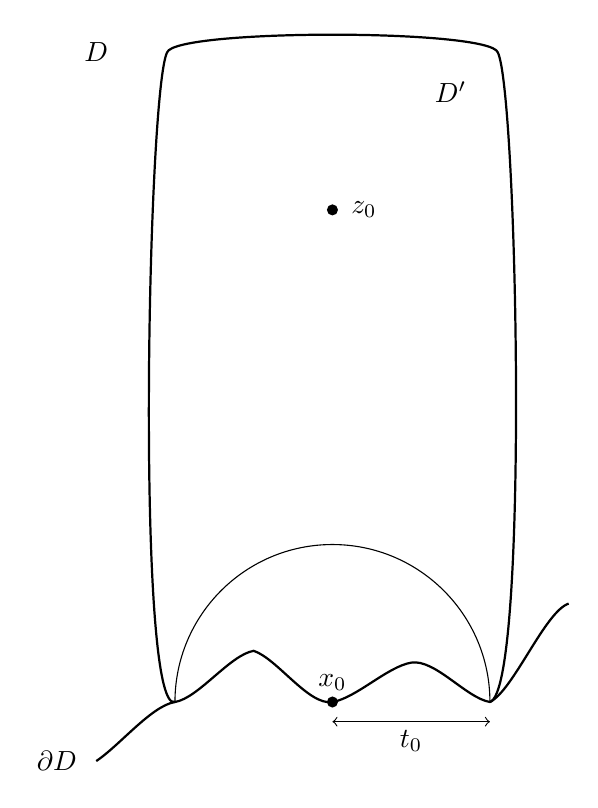
\begin{tikzpicture}
			% Main curve as cubic Bézier segments
			\draw[thick]
			(-3,-1)
			.. controls (-2.7,-0.8) and (-2.3,-0.3) ..
			(-2,-0.25)
			.. controls (-1.7,-0.2) and (-1.3,0.35) ..
			(-1,0.4)
			.. controls (-0.7,0.30) and (-0.3,-0.30) ..
			(0,-0.25)
			.. controls (0.3,-0.20) and (0.7,0.20) ..
			(1,0.25)
			.. controls (1.3,0.30) and (1.7,-0.2) ..
			(2,-0.25)
			.. controls (2.3,-0.1) and (2.7,0.9) ..
			(3,1);
			
			% Branch
			\draw[thick]
			(-2,-0.25)
			.. controls (-2.5,-0.4) and (-2.35,7.5) ..
			(-2.10,8)
			.. controls (-2,8.3) and (2,8.3)..
			(2.1,8)
			.. controls (2.35,7.5) and (2.5,-0.1)..
			(2,-0.25);
			
			\fill (0,-0.25) circle (2pt);
			\node at (0,0){$x_0$};
			\fill (0,6) circle (2pt);
			\node at (0.4,6){$z_0$};
			
			\draw (2,-0.25) arc[start angle=0,end angle=180,radius=2];
			
			\draw[<->] (0,-0.5)--(2,-0.5);
			\node at (1,-0.75){$t_0$};
			
			\node at (-3,8){$D$};
			\node at (1.5,7.5){$D'$};
			\node at (-3.5,-1){$\partial D$};
		\end{tikzpicture}
		\caption{The star-shaped $C^{1,\mathrm{Dini}}$ domain $D'$ with center $z_0$. }
	\end{figure}

	\begin{theorem}\label{thm:BogdanLD}
		Let $D\subset\mathbb R^d$ be a $C^{1,\mathrm{Dini}}$ domain. Then
		\begin{align}\label{eq:GreenFuncEstLD}
			G(x,y)\sim|x-y|^{2-d}\left(\frac{\delta(x)}{|x-y|}\wedge 1\right)\left(\frac{\delta(y)}{|x-y|}\wedge 1\right)
		\end{align}
		and
		\begin{align}\label{eq:MartinKernelDiniDom}
			k^{z_0}(z,\xi)\sim\frac{\delta(z)}{|z-\xi|}\left(\frac{|z-\xi|}{|z_0-\xi|}\right)^{1-d}
		\end{align}
	\end{theorem}

	\begin{lemma}\label{lem:quasisymm}
		Let $D$ be a Lipschitz domain with character $(\rho_0,M)$ and let $r<\rho_0$ and $\xi,\zeta\in\partial D$. Then
		\begin{align*}
			\frac{k(A_r(\xi),\zeta)}{k(A_r(\zeta),\xi)}\sim\frac{G(A_r(\xi),0)}{G(A_r(\zeta),0)}.
		\end{align*}
		In particular, if the domain is $C^{1,\mathrm{Dini}}$, $k(A_r(\xi),\zeta)\sim k(A_r(\zeta),\xi)$.
	\end{lemma}

	\begin{lemma}\label{lem:harmeasVShausdorff}
		
		Let $D$ be a $C^{1,\mathrm{Dini}}$ domain with $\delta(0)\geq 2\rho_0$. There exists a constant $C=C(D)>0$, such that
		\begin{align}\label{eq:EquivalenceOfMeasures}
			C^{-1}\leq\frac{\omega(A)}{\mathcal{H}^{d-1}(A)}\leq C
		\end{align}
		for any Borel set $A\subset\partial D$.
		In particular, 
		\begin{align*}
			C^{-1}\leq\frac{k(z,\xi)}{p(z,\xi)}\leq C
		\end{align*}
		for all $z\in D$ and $\xi\in\partial D$.
	\end{lemma}

	\begin{theorem}\label{thm:MainThm1}
		If $D\subset\mathbb R^d$ is a $C^{1,\mathrm{Dini}}$ domain and $u\geq0$ is harmonic on $D$, there exists $\xi\in\partial D$ such that 
		\begin{align}\label{eq:FullVar}
			V(\xi,u)=\int_D|\nabla u(z)|p(z,\xi)\mathrm{d}z<\infty
		\end{align}
		In fact, the set $\mathcal B(u, D):=\lbrace\xi\in\partial D: V(\xi,u)<\infty\rbrace$ is ultradense in $\partial D$, i.e. for every ball $B$ that has its center on $\partial D$, $\dim \mathcal{B}(u,D)\cap B=d-1$.	
	\end{theorem}

	\begin{proof}[Proof of Theorem \ref{thm:MainThm1}]:\newline
		\textbf{Step 1:} Assume that $D$ is star-shaped. Define the function $r(z):=|z|/|\Phi(z/|z|)|$ and check that $r^{-1}(\lbrace t\rbrace)=t\partial D$, $t\in(0,1)$. Write $\theta=z/|z|$ and $\Phi=(\phi_j)_j$. Compute 
		\begin{align*}
			\partial_i r(z) = \frac{z_i}{|z||\Phi(\theta)|}-\frac{1}{|\Phi(\theta)|^3}\sum_j\phi_j(\theta)\sum_k(\partial_k\phi_j)(\theta)\left(\delta_{ik}-\frac{z_iz_k}{|z|^2}\right),
		\end{align*}
		so by orthogonality of the two vectors, $|\nabla r(z)|^2\geq1/|\Phi(\theta)|^2$. In total $|\nabla r|\sim_\Phi 1$, by our assumptions on the function $\Phi$.
		Applying the coarea formula yields
		\begin{align}\label{eq:Coarea}
			\begin{aligned}
				\int_{D}|\nabla u(z)|k(z,\xi)|\nabla r(z)|\mathrm{d}z&=\int_0^1\int_{t\partial D} |\nabla u(\zeta)|k(\zeta,\xi)\mathrm{d}\mathcal{H}^{d-1}(\zeta)\mathrm dt\\
				&=\int_0^{1}(1-t)^{d-1}\int_{\partial D}|\nabla u(\zeta_t)|k(\zeta_t,\xi)\mathrm{d}\mathcal{H}^{d-1}(\zeta)\mathrm{d}t
			\end{aligned}
		\end{align}
		Lemma \ref{lem:quasisymm} implies,
		\begin{align}\label{eq:quasisymm}
			k(\zeta_t,\xi)\sim k(\xi_t,\zeta)
		\end{align}
		for $t\leq r_0$. If $t>r_0$, we obtain \eqref{eq:quasisymm} by Harnack's inequality. Plugging \eqref{eq:quasisymm} into the right side of \eqref{eq:Coarea} and replacing surface measure by harmonic measure yields
		\begin{align}\label{eq:RadImpliesFull}
				\int_{D}|\nabla u(z)|k(z,\xi)\mathrm{d}z\sim \int_0^{1}\int_{\partial D}|\nabla u(\zeta_t)|k(\xi_t,\zeta)\mathrm{d}\omega(\zeta)\mathrm{d}t
		\end{align}
		by Lemma \ref{lem:harmeasVShausdorff}. The right side of \eqref{eq:RadImpliesFull} is finite for any $\xi\in\mathcal B_{\mathrm{rad}}(u,D)$, so $\mathcal B_{\mathrm{rad}}(u,D)\subset \mathcal B(u, D)$ implying the desired statements about ultradensity.\\\\
		\textbf{Step 2:} Assume $D$ is not star-shaped. This step is proved by covering a neighborhood of the boundary with finitely many star-shaped $C^{1,\mathrm{Dini}}$ domains and applying Step 1. \par 
		Recall from the proof of Theorem \ref{thm:MainThm2} that there exist scalars $t_0,b>0$ such that for any $x_0\in\partial D$, there exists a star-shaped $C^{1,\mathrm{Dini}}$ domain $D(x_0)\subset D$ satisfying $B(x_0,t_0)\cap D\subset D(x_0)$ and its center $z_0$ satisfies $\delta_D(z_0)\gtrsim bt_0$ (see figure \ref{fig:D'}). Let $B=B(x_0,r)$ be a ball with center $x_0\in\partial D$ and radius $r<t_0/8$. Our goal is to prove $\dim\mathcal B(u,D)\cap B=d-1$. Construct the domain $D(x_0)$ as above and call it $D_0$ with center $z_0$. By Step 1, $\dim \mathcal B(u,D_0)\cap B=d-1$. It suffices to prove that $\mathcal B(u,D_0)\cap B\subset \mathcal B(u, D)\cap B$ i.e. we have to prove that
		\begin{align}
			\forall \xi\in B\cap\partial D:\quad\int_{D_0}|\nabla u(z)| p_{D_0}(z,\xi)\mathrm dz<\infty\Rightarrow\int_{D}|\nabla u(z)|p(z,\xi)\mathrm dz<\infty,
		\end{align}
		where $p_{D_0}$ denotes the local Poisson kernel on the domain $D_0$. Fix some $\xi\in B\cap\partial D$ with
		\begin{align*}
			\int_{D_0}|\nabla u(z)| p_{D_0}(z,\xi)\mathrm dz<\infty.
		\end{align*}
		\textbf{Covering argument: }There exist $c=c(D)>0$ and $x_1,\dots x_N\in\partial D$ satisfying $|x_i-x_0|\geq3/4t_0$ such that
		\begin{align}
			B(x_0,t_0/2)\cup\bigcup_{i=1}^N B(x_i,t_0/2)\supset \lbrace z\in D:\delta(z)<c\rbrace.
		\end{align}
		This can be achieved by covering $\partial D\setminus B(x_0,3/4t_0)$ with finitely many balls of radius $t_0/K$, $K\gg1$. Then take the balls with the same centers but radius $t_0/2$. For each $x_i$ construct the star-shaped $C^{1,\mathrm{Dini}}$ domains $D_i=D(x_i)$ with centers $z_i\in D$, satisfying $\delta_D(z_i)>bt_0$. Note that by their definition, $B_i\cap D\subset D_i$, where $B_i:=B(x_i,t_0/2)$. Applying Step 1 to each of the $D_i$, $i>0$, there exist $\xi_i\in B_i\cap\partial D$ such that
		\begin{align}
			\int_{D_i}|\nabla u(z)|p_{D_i}(z,\xi_i)\mathrm dz<\infty.
		\end{align}
		Note that
		\begin{align}\label{eq:JonesSplitting}
			\int_{D}|\nabla u(z)|p(z,\xi)\mathrm dz&\leq\int_{B_0\cap D}|\nabla u(z)|p(z,\xi)\mathrm dz+ \sum_{i=1}^{N}\int_{B_i\cap D}|\nabla u(z)|p(z,\xi)\mathrm dz\\
			&+\int_{\lbrace\delta(z)\geq c\rbrace}|\nabla u(z)|p(z,\xi)\mathrm dz\label{eq:finiteIntegral}
		\end{align}
		\textbf{Behavior of local Poisson kernels:} We investigate the behavior of the local Poisson kernels $p_{D_i}$ and the global Poisson kernel $p$ on the sets $B_i\cap D$. We begin by bounding the left term in \eqref{eq:JonesSplitting}.
	 	By Theorem \ref{thm:BogdanLD}
		\begin{align}\label{eq:localMartinKernel}
			k^{z_0}_{D_0}(z,\xi)\sim\frac{\delta_{D_0}(z)}{|z-\xi|^d}|z_0-\xi|^{d-1}\sim k^{z_0}_{D}(z,\xi),
		\end{align}
		since $\delta_{D_0}(z)\sim\delta(z)$ for $z\in B_0\cap D$.
		Apply \eqref{eq:localMartinKernel} and recall the factorization 
		\begin{align*}
			p_{D_0}(z,\xi)=p_{D_0}(z_0,\xi) k^{z_0}_{D_0}(z,\xi)\sim p_{D_0}(z_0,\xi)k^{z_0}_{D}(z,\xi) = \frac{p_{D_0}(z_0,\xi)}{p(z_0,\xi)} p(z,\xi).
		\end{align*} 
		Therefore 
		\begin{align}
			\int_{B_0\cap D}|\nabla u(z)|p(z,\xi)\mathrm dz \sim \frac{p(z_0,\xi)}{p_{D_0}(z_0,\xi)} \int_{B_0\cap D}|\nabla u(z)|p_{D_0}(z,\xi)\mathrm dz<\infty
		\end{align}
		
		We now turn to the right term in \eqref{eq:JonesSplitting}. Fix $i=1,\dots,N$, and $z\in B_i\cap D$, then $|z-\xi|\gtrsim|z-\xi_i|$. This follows from the inequalities $|z-\xi_i|\leq t_0$ and 
		\begin{align}
			|z-\xi|\geq|x_i-x_0|-|z-x_i|-|\xi-x_0|\geq t_0/8
		\end{align}
		Moreover $|z_i-\xi|\leq\mathrm{diam}(D)$ and $|z_i-\xi_i|\geq\delta(z_i)\geq b t_0$, so in total $|z_i-\xi|\lesssim|z_i-\xi_i|$ Once again Theorem \ref{thm:BogdanLD} implies
		\begin{align}\label{eq:MartinKernelEstimateD_i}
			k_{D}^{z_i}(z,\xi)\sim\frac{\delta(z)}{|z-\xi|^d}|z_i-\xi|^{d-1}\lesssim \frac{\delta(z)}{|z-\xi_i|^d}|z_i-\xi_i|^{d-1}\sim k_{D_i}^{z_i}(z,\xi_i).
		\end{align}
		We use inequality \eqref{eq:MartinKernelEstimateD_i} in
		\begin{align*}
			p(z,\xi)=p(z_i,\xi) k^{z_i}_{D}(z,\xi)\lesssim p(z_i,\xi)k^{z_i}_{ D_i}(z,\xi_i) = \frac{p(z_i,\xi)}{p_{D_i}(z_i,\xi_i)} p_{D_i}(z,\xi_i),
		\end{align*}
		implying 
		\begin{align}
			\int_{B_i\cap D}|\nabla u(z)|p(z,\xi)\mathrm dz\lesssim \frac{p(z_i,\xi)}{p_{D_i}(z_i,\xi_i)}\int_{B_i\cap D}|\nabla u(z)|p_{D_i}(z,\xi_i)\mathrm dz<\infty.
		\end{align}
		This completes the proof since the integral in \eqref{eq:finiteIntegral} is finite.
	\end{proof}

\end{document}
